\section{Plotting a learning curve}

This section describes how training progress was monitored by plotting a learning curve.

\subsection{Previous corpora and their problems}

The following two corpora were available for training from the IP8 project.

\begin{itemize}
	\item \textbf{\ac{LS}}: This corpus was created as an artifact of the IP8 project using raw data from OpenSLR. The raw is publicly available and can be downloaded\footnote{\url{http://www.openslr.org/12/}}. It consists of a number of audio files which were \textit{partially} transcribed, i.e. there are parts in the audio for which the corresponding transcript is not exactly known (the audio contains \textit{gaps}). The individual samples were obtained by exploiting metadata that was included in the download. The metadata includes a split into a training set (containing approximately 96\% of the samples) and a validation resp. test set (each containing approximately 3\% of the samples). The split was done manually into disjoint subset, i.e. ensuring each speaker was only included in one set. Additionally, other features like gender or accent were observed to achieve a similar distribution for each set. To leverage the efforts made by \textit{OpenSLR}, this split was not changed.
	\item \textbf{\ac{RL}}: This corpus was created from raw data provided by \textit{ReadyLingua}. This data is proprietary and contains recordings in several languages which were manually aligned with their transcript. In contrast to the \ac{LS} corpus, the raw data is fully aligned, i.e. there are no gaps in the audio. However, the metadata does not comprise a split into training-, validation- and test-set. Since the raw data contained recordings and transcripts in more than one language, separate splits were made for each language preserving a ratio of approximately 80/10/10\% (relating to the total length of all recordings within each subset). Efforts were made to prevent samples from the same recording being assigned to different subsets. Other features were not observed, meaning the split into train/validation/test-set was done less carefully than in the \ac{LS} corpus.
\end{itemize}

The model in the IP8 project was supposed to be trained on the \ac{LS} corpus, because this corpus is much larger than the \ac{RL} corpus. In the course of the project it became clear however that training on all samples from this corpus was not feasible within project time because training time would have taken more than two months. It also turned out that the \ac{LS} corpus was probably less useful than initially assumed because the average sample length was much longer than the samples in the \ac{RL} corpus. This made training even harder because convergence is much slower when training on long sequences. The \ac{RL} corpus on the other hand consisted of shorter samples, but the total length of all samples was only a few hours compared to the 1000+ hours in the \ac{LS} corpus.

\subsection{The \textit{CommonVoice} Corpus}

Because of the aforementioned problems a new corpus was needed which combined the best of both worlds:

\begin{itemize}
	\item it should contain a reasonable amount of speech samples to facilitate training an ASR model
	\item the average sample length should be short enough for the model to learn quickly.
\end{itemize}

The \ac{CV}\footnote{\url{https://voice.mozilla.org/en/data}} corpus is maintained and used actively by the Mozilla Foundation and exhibits both of these properties. This corpus is also used to train the Mozilla implementation of \textit{DeepSpeech}. Datasets for various languages are being prepared and verified, each one containing speech samples of different contributors from all over the world. At the time of this writing, only the English dataset was available, but datasets for other languages will become publicly available at some time in the future. The English dataset comes pre-divided into training-, validation- and test-set of similar scale like the \ac{LS} corpus. Each set consists of one audio file per sample and a CSV file containing the transcriptions for each sample.

The simplified model in this project was trained on the training-set of the \ac{CV} corpus. Although still smaller than than the \ac{LS} corpus, the total length of all validated samples that can be used for training\footnote{CSV file: \code{cv-valid-train.csv}} is much larger than the \ac{RL} corpus while providing samples of similar length at the same time. Table \ref{corpora_stats} shows some statistics about the corpora described above.

\begin{table}[!htbp]
	\centering
	\begin{tabular}[t]{llrrrrr}
		\toprule
		\thead{Corpus} & \thead{Language} & \thead{total audio length} & train/dev/test & \thead{\# samples} & \thead{Ø sample\\length (s)} & \thead{Ø transcript\\length (chars)} \\
		\midrule
 		\ac{LS} & English & $24 days, 7:13:18$ & $93.51/3.32/3.16\%$ & $166,510$ & $12.60$ & $183.84$ \\ 
		\ac{RL} & English & $5:38:39$ & $80.39/10.13/9.48\%$ & $6,334$ & $3.20$ & $51.81$ \\ 		
		\ac{RL} & German & $1:58:30$ & $81.14/10.26/8.60\%$ & $2,397$ & $2.89$ & $45.55$ \\ 		
		\ac{CV} & English & $10 days, 1:02:53$ & $96.04/1.99/1.98\%$ & $201,252$ & $4.31$ & $48.07$ \\ 
		\bottomrule
	\end{tabular}
	\caption{Statistics about corpora that were available for training.}
	\label{corpora_stats}
\end{table}

\subsection{Plotting the learning curve}

The time needed to train an \ac{ASR} model on all samples of the \ac{CV} corpus is still too long for the available project time. We can however still get an estimate of the learning progress by plotting a \textit{learning curve}. For this, exponentially increasing amounts of training data (1, 10, 100 and 1,000 minutes of transcribed audio) were used. Training was done making 30 full passes over the training set (\textit{epochs}). The training samples were processed in batches of 16 samples each. They were sorted by the length of their audio signal and then zero-padded\footnote{sorting the samples was done to have sequences of similar length in each batch and thus reduce padding}, yielding samples of the same length in each batch\footnote{note that the length of the samples could still vary between batches}. 

After each epoch, the progress was monitored by inferring the transcriptions for previously unseen samples from the validation set. The \ac{CTC}-loss for training and validation was plotted for each amount, yielding separate curves for the training- and the validation-loss. Comparing both curves allows for making statements about at what point the Neural Network starts to overfit.

Complementary to the \ac{CTC}-loss, the mean values for the \ac{LER} and \ac{WER} metric over all samples in the validation set was calculated after each epoch, yielding the curves for the \ac{LER} resp. \ac{WER}. Observing these plots can give some insight about how well the network performs on unseen examples.

Both loss and metrics were compared along two dimensions:

\begin{itemize}
	\item \textbf{The decoder dimension}, comparing the two distinct ways to decode a transcript from the probability distributions calculated by the model for each frame in the input signal
	\item \textbf{The LM dimension}, comparing inferences made with and without post-processing the decoded transcript with a spell-checker as described above
\end{itemize}

Both dimensions are described in more detail below.

\subsubsection{Decoder dimension}

In a nutshell, \ac{CTC} aligns the $T_y$ characters from a known transcription (\textit{label} or \textit{ground truth}) with the $T_x$ frames from the input audio signal during training. $T_x$ is typically much larger than $T_y$ and must not be shorter. The characters (\textit{tokens}) in the label must come from an alphabet of size $V$, which for English are the 26 lowercased ASCII characters $a..z$, the space character and the apostrophe (because this character is very common in contracted words like e.g. \textit{"don't"} or \textit{"isn't"}). Additionally, \ac{CTC} introduces a special token $\epsilon$, called the \textit{blank token}, which can be used to label unknown/silent frames or prevent collapsing (see below). Consequently, the number of characters in the alphabet used by the \ac{ASR} in this project to recognize English is $|V|=26+1+1+1=29$.

\ac{CTC} is \textit{alignment-free}, i.e. it does not require an alignment between the characters of a transcription and the frames of an audio signal. The only thing needed is the audio signal $X$ itself plus its ground truth $Y$. Each token in the ground truth can be aligned with any number of frames in the input signal. Vice versa, repeated sequences of the same characters can be collapsed, whereas the $\epsilon$ token acts as a boundary within sequences of a token to prevent collapsing into one, when there should be two (such as in \textit{f-f-o-o-$\epsilon$-o-o-o-o-d-d-d}, which should collapse to \textit{food} and not \textit{fod}). 

For each frame input signal \ac{CTC} calculates a probability distribution over the $|V|$ characters in the alphabet. This yields a $|V| \times T_x$ probability matrix for the input signal. Because $T_x \ggg T_y$, there is usually a vast amount of different valid alignments collapsing to the same ground truth. The probability of each valid alignment can now simply be calculated by traversing the probability matrix from left to right and multiplying the probabilities of each character. Because calculating the probability of each valid alignment individually would be too slow and identical prefixes between valid alignments yield identical probabilities, a dynamic programming approach is usually chosen to calculate the probabilities whereas the intermediate probability for each prefix is saved once computed.

The most probable alignment is calculated by marginalizing (i.e. summing up) over the probabilities of the individual valid alignments. This calculation yields the CTC loss as a sum of products, which is differentiable and can therefore be optimized.

After training, a model using \ac{CTC} will again output a $|V| \times T_x$ probability matrix for any previously unseen input. This matrix can be used to infer a transcription, a process also known as \textit{decoding}. The \ac{CTC} paper proposes two different decoding strategies that are applied before collapsing the characters \cite{ctc_paper}:

\begin{itemize}
	\item \textbf{Best-Path (a.k.a. \textit{greedy}) decoding}: This strategy only ever considers the most likely character at each time step. The transcription before collapsing will be a single path through the the probability matrix, whose probability will be the product of all elements along the path. This approach is easy to implement but does not take into account the fact that a single output can have many alignments, whose individual probability may be lower than the one found with this strategy.
	\item \textbf{Beam-Search decoding}: This strategy approximates the probability of the most probable transcription by following multiple paths simultaneously and only keeping the $B$ most probable paths at each time step. The beam width is a hyperparameter that can be increased to get a more accurate transcription in exchange for higher computational cost.
\end{itemize}

Beam-Search decoding is expected to perform better. For the sake of completeness, both decoding strategies were compared in this project. This will yield separate learning curves for the decoder dimension. For Beam-Search decoding, the Keras implementation was used, which proposes a default beam width of $B=100$. This value was not changed. 

\subsubsection{\ac{LM} dimension}

Using a \ac{LM} to post-process the inferred transcription with a rudimentary spell checker will not necessarily lead to more accurate transcription, especially if the edit distance between prediction and ground truth is large. Table \ref{lm_bad_example} contains an example where the use of a spell checker is disadvantageous to the quality of a transcription.

\begin{table}[!htbp]
	\centering
	\begin{tabular}{llr}
		\toprule
		 &  & \thead{\ac{LER}} \\
		\midrule
		\textbf{ground truth} & i want to wish you a very happy thanksgiving & \\ 
		\textbf{prediction before spell-checking} & oento wiceyouepery appy thangksive & 0.4318 \\ 
		\textbf{prediction after spell-checking} & onto wiceyouepery app thangksive & 0.4545 \\ 		
		\bottomrule
	\end{tabular}
	\caption{Example of a transcription whose \ac{LER} was increased when using a spell checker}
	\label{lm_bad_example}
\end{table}

%ground truth: i want to wish you a very happy thanksgiving	
%prediction: oento wiceyouepery appy thangksive (LER=0.431818181818182, WER=1)
%prediction (LM-corrected): onto wiceyouepery app thangksive	(LER=0.454545454545455	WER=1)

%\begin{figure}[h!]
%	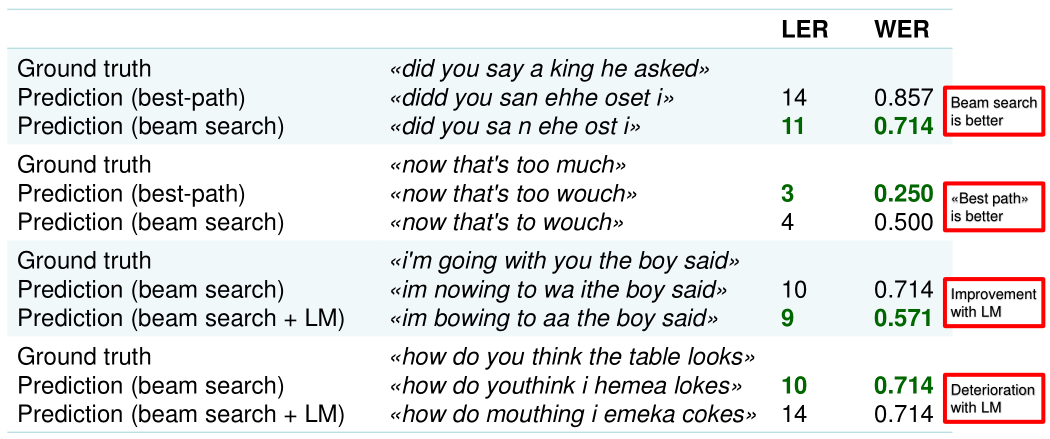
\includegraphics[width=\linewidth]{./img/lm_dimension_example.png}
%	\caption{Example of how a spell checker can improve or deteriorate the quality of a prediction.}
%	\label{lm_dimension_example}
%\end{figure}

In this example, \foreignquote{french}{\textit{oento}} was changed to \foreignquote{french}{\textit{onto}} because this was the most probable word with a maximum edit distance of 2 that was in the vocabulary. Similarly, \foreignquote{french}{\textit{appy}} was changed to \foreignquote{french}{\textit{app}}. This lead to a orthographically better sentence, but the \ac{LER} is higher than without spell-checking. 

It is generally expected that post-processing the inference as described above will lead to a lower \ac{WER}, supposed the \ac{LER} is already low enough, i.e. the prediction matches the ground truth already pretty well. If the \ac{LER} value is too high, the spell checker might try too hard to find a word from the vocabulary. This might result in a changed sentence consisting of real words but whose similarity to the ground truth is lower than before the changes. Post-processing might then be counter-productive. Therefore, separate learning curves were plotted for inference with and without post-processing (the \textit{\ac{LM} dimension})

\subsection{Results and interpretation}

Figure \ref{lc_loss_cv} shows the learning curve for the \ac{CTC}-loss. Obviously the training loss decreases steadily for all amounts of training data, converging to values between 30 (training on $1.000$ minutes) and 50 (training on 1 minute). Because the network does not generalize well when being trained on only 1 or 10 minutes of audio data, its predictions are somewhat random. This may be an explanation for the jagged curve of the validation plot (dashed lines) for these amounts of training data. When training on 100 minutes, the plot for the validation loss is smoother, but starts to increase between epoch 10 and 15, meaning the network starts to overfit after that point. When training on 1.000 minutes the validation loss does not decrease after epoch 14 anymore and plateaus at a value of about 90, meaning that any training will not contribute to a more generalizable network.

\begin{figure}[h!]
	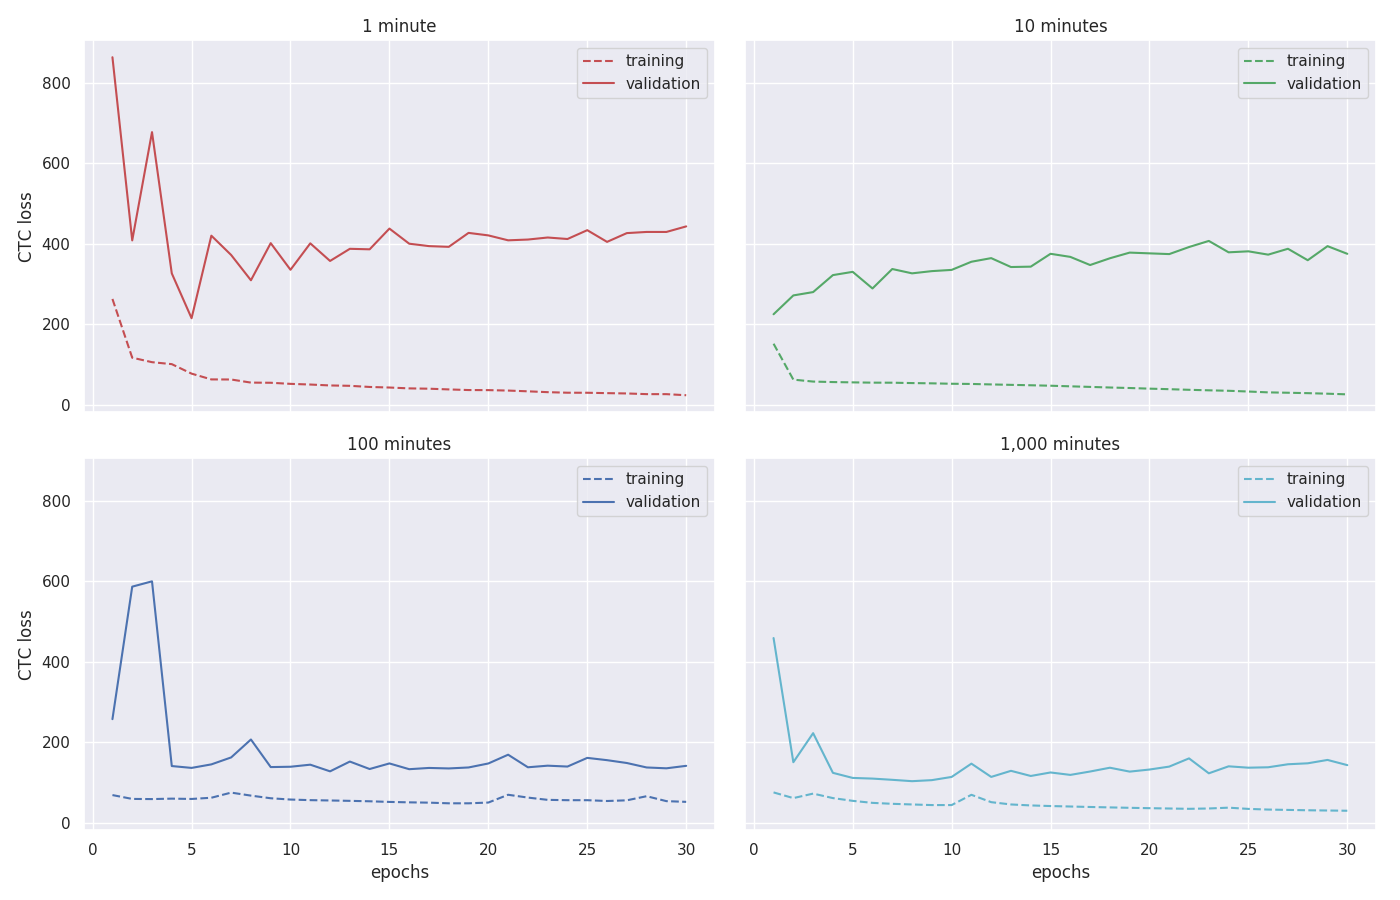
\includegraphics[width=\linewidth]{./img/lc_loss_cv.png}
	\caption{Learning curve for the CTC-loss while training on 1/10/100/1000 minutes of transcribed audio from the \ac{CV} corpus using the $5$-gram \ac{LM} provided by the Mozilla implementation of \textit{DeepSpeech}}
	\label{lc_loss_cv}
\end{figure}

Figure \ref{lc_ler_cv} shows how the average values of the \ac{LER} over all validation samples develops for the different amounts of training data. The plot on the left shows the results when using best-path decoding, the plot on the right for beam search decoding. The plots for all amounts of training data have been integrated in the same plot for the sake of a clearer representation. Both plots support the conclusions made for the CTC loss in that -- except when training on 1.000 minutes of audio -- the error rates do not decrease after epoch 15 anymore (in fact there is a slight increase). The plots for the \ac{LER} when training on 1.000 minutes are almost identical for both decoding strategies. Surprisingly, the \ac{LER} values continue to decline steadily, although only at a very slow rate, finishing with values of 0.54 (best-path decoding) resp. 0.52 (beam search decoding), meaning that the network got a bit more than half of the characters wrong, at the wrong position or entirely failed to predict them. The values when trying to correct the inferred transcriptions with a spell checker are slightly higher for both decoding strategies (0.55 and 0.53) meaning that post-processing did not help. This nourishes the assumption that a spell checker will probably only lower the \ac{WER} and only do so if the \ac{LER} is already low enough (see above).

\begin{figure}[h!]
	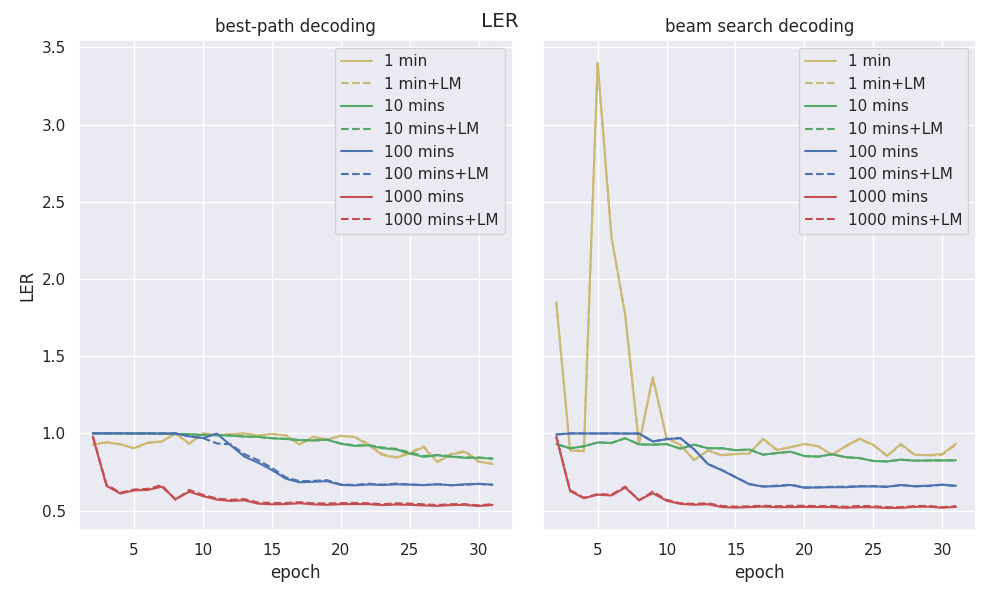
\includegraphics[width=\linewidth]{./img/lc_ler_cv.png}
	\caption{Learning curve for the \ac{LER} metric while training on 1/10/100/1000 minutes of transcribed audio from the \ac{CV} corpus with and without spelling correction with a \ac{LM}. For the lines where spelling was corrected, the $5$-gram \ac{LM} provided by the Mozilla implementation of \textit{DeepSpeech} was used.}
	\label{lc_ler_cv}
\end{figure}

Finally, figure \ref{lc_wer_cv} shows the development of the average \ac{WER} values over all validation samples. Not surprisingly, the plots oscillate around a value of 1, meaning the network did not get any of the words right. Only when training on 1.000 minutes, the network was able to achieve a value below 1, but is still way higher than the 0.0065 achieved by the Mozilla implementation of \textit{DeepSpeech}. It is noteworthy that the use of a spell checker marginally improves the results here.

\begin{figure}[h!]
	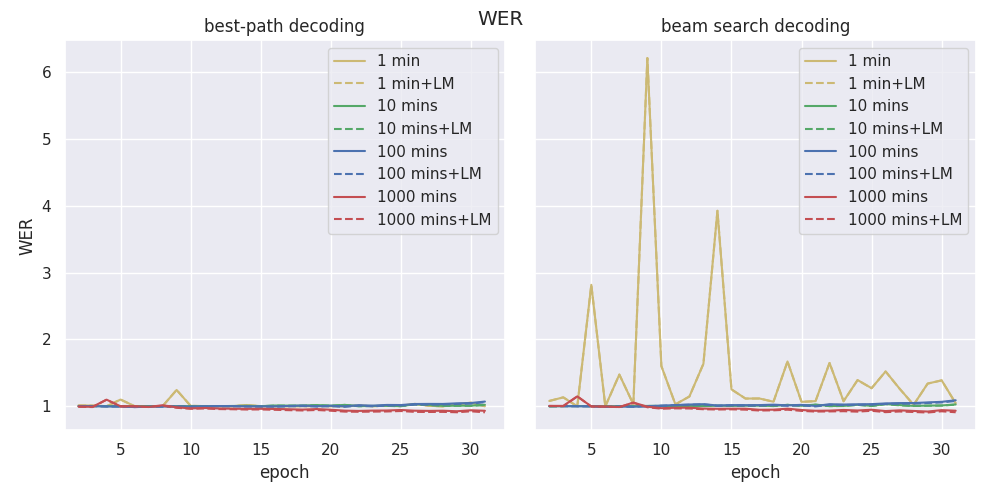
\includegraphics[width=\linewidth]{./img/lc_wer_cv.png}
	\caption{Learning curve for the \ac{WER} metric while training on 1/10/100/1000 minutes of transcribed audio from the \ac{CV} corpus with and without spelling correction with a \ac{LM}. For the lines where spelling was corrected, the $5$-gram \ac{LM} provided by the Mozilla implementation of \textit{DeepSpeech} was used.}
	\label{lc_wer_cv}
\end{figure}

In summary it can be said that the lowest \ac{LER} rates can be achieved when training on $1.000$ minutes of audio, not using the spell-checker. Training can be stopped after about 15 epochs however, because the results on validation data does not improve from there on. The average \ac{LER} of $0.52$ suggests that the network predicts about half of the characters right. This yields transcriptions which -- although far from correct -- are recognizeable as human language. Sometimes the real transcript might be guessed, especially for shorter sentences. Table \ref{training_progress} shows an example for how the accuracy of the inferred transcript improves with additional training data.

\begin{table}[!htbp]
	\centering
	\begin{tabular}{llll}
		\toprule
		\thead{training data} & \thead{inferred transcript} & \thead{\ac{LER}} \\
		\midrule
		1 minute & w t e isi & $0.76$  \\ 	
		10 minutes & tiar n th i id & $0.71$  \\ 		
		100 minutes & ave gos goe ei & $0.52$  \\ 		
		1.000 minutes & i've got go fi ha & $0.33$  \\ 		
		\bottomrule
	\end{tabular}
	\caption{Example of how the quality for inferred transcripts improves with additional training data. The \ac{LER} values were calculated against the ground truth \foreignquote{french}{\textit{i've got to go to him}}}
	\label{training_progress}
\end{table}

\subsection{Regularization}
As an attempt to prevent overfitting (or at least postpone it to later epochs), the network has been regularized by adding dropouts after each layer. The rate of each dropout has been set to 0.1, meaning a random 10\% of the unit weights in each layer will be zeroed out. Apart from adding dropouts no further changes were made to the simplified model.

The learning curve for the model with dropouts is similar to the one without dropouts, meaning its validation loss will plateau after about 15 epochs. To compare the simplified model with and without dropout, the average \ac{LER} on the \ac{CV} test-set was calculated with both decoding strategies. Table \ref{comparison_regularized_unregularized} shows the results of the comparison. The observations made for the spell checker also apply to the model with dropouts, meaning that the \ac{LER} rate is slightly better without spell-checking. The lowest average \ac{LER} rate (highlighted) was achieved using beam search and no spell checker. Although the difference is only marginal, the regularized model will be used for further evaluation.

\begin{table*}\centering
	\ra{1.3}
	\begin{tabular}{@{}rrrrcrrrcrrr@{}}\toprule
		& \multicolumn{2}{c}{Ø $LER$} \\
		\cmidrule{2-3}
		& not regularized & regularized\\ \midrule
		\textbf{best-path decoding}\\
		without spell-checker & 0.5359 & 0.5343 \\
		with spell-checker & 0.5475 & 0.5456 \\
		\textbf{beam search decoding}\\
		without spell-checker & 0.5146 & \cellcolor{green!25}0.5125 \\
		with spell-checker & 0.5256 & 0.5242 \\
		\bottomrule
	\end{tabular}
	\caption{Comparison of the simplified model with and without dropout regularization. The average \ac{LER} was calculated over all samples from the \ac{CV} test-set. The best value is highlighted.}
	\label{comparison_regularized_unregularized}
\end{table*}

%Figure \ref{lc_regularization_cv} show the difference between the original simplified model and the same model with dropouts added. Only the plots for training on $1.000$ are shown. Decoding was done using Beam-Search decoding. The plot on the left shows how the training/validation-loss develops for each model. The plot on the right shows how the average \ac{LER} on the validation set develops for each model.

%\begin{figure}[h!]
%	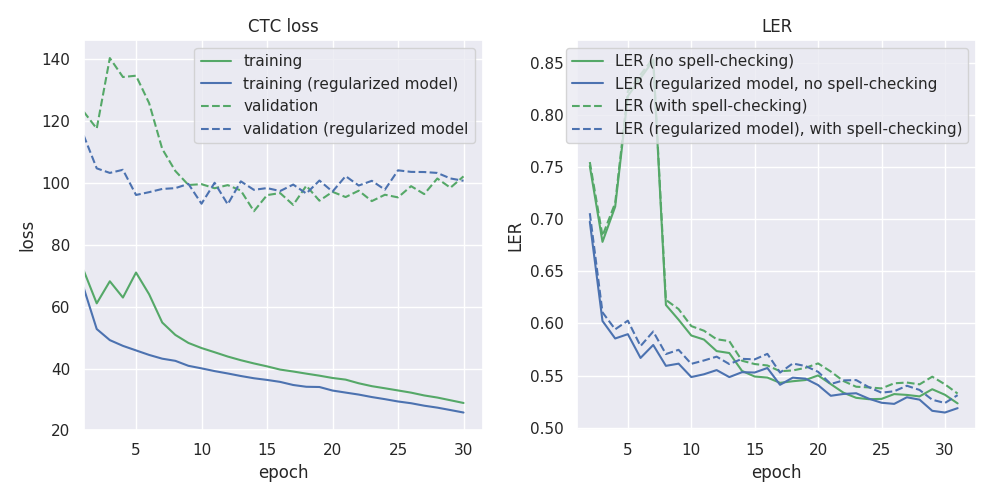
\includegraphics[width=\linewidth]{./img/lc_regularization_cv.png}
%	\caption{\ac{CTC}-loss and \ac{LER} values when training a simplified model with and without regularization. Apart from adding dropouts, no further changes were made to the original model. $1.000$ minutes of training data from the \ac{CV} corpus were used for training.}
%	\label{lc_regularization_cv}
%\end{figure}

\subsection{Final thoughts and considerations}

Above results were achieved with a spell checker using a vocabulary of 80.000 words and the 5-gram \ac{LM} from Mozilla. This did not help very much, but it might be possible that a different vocabulary size will produce better results. It is also possible that a different Optimizer, different dropout rates or integrating the \ac{LM} score into the cost function (like Mozilla did) will produce better results. Finally, it might be fruitful to train on smaller batches as it has been observed by \cite{batch_size_rnn} that with larger batches the quality of a model degrades. 

All these ideas produces many more combinations to try out, but preparing and running them is very time consuming. Because the \ac{LER} of about 0.5 (1.000 minutes, no spell checker) looks promising, I decided to leave it at this for the moment and see how far I get.

\subsubsection{Summary}

This chapter gave a quick introduction into how \ac{CTC} and its different decoding strategies work. It also gave an overview over the available corpora and showed how the training progress developed with varying amounts of training data, different decoding strategies and the use of a spell-checker. Post-processing the inferences with a spell-checker will not always lead to better transcripts. Training was done using samples from the \textit{CommonVoice} corpus. A regularized model was created by adding dropouts to the simplified model. The best results were obtained with the regularized model not using the spell-checker. When training this model on $1.000$ minutes of data the average \ac{LER} on test data is only slightly higher than $0.5$, meaning the model will get about 50\% of the characters in the transcript right. However it was also observed that both the regularized and unregularized model start to overfit after about 15 epochs.